\textbf{\textit{The Models}}---
As an example, we will consider the Majoron model. Nevertheless the study can also be applied to sterile neutrinos via magnetic portal. For the case of sterile neutrino with mixing portal, special care needs to be taken for resonant conversions in which case active neutrinos with plasma mass would travel as slowly as the sterile neutrinos at specific distances.
The relevant part of the Lagrangian in the Majoron case reads
\begin{align}
\mathcal{L} \supset -\frac{g_{\alpha\beta}}{2} \nu_\alpha \nu_\beta \phi - M_\phi \phi\phi^* + \text{h.c.}\,,
\end{align}
where $M_\phi$ is the Majoron mass and $g$ parametrizes interaction strength between $\phi$ and neutrinos. Consider flavor universal interaction, we abbreviate $g_{\alpha\beta}\equiv g$. Majorons are produced from neutrino coalescence in the star and then subsequently decay to a pair of neutrinos with the total decay width to all flavor of neutrinos given by $\Gamma_\phi = 3g^2 m_\phi/16 \pi$, and as a result, BSM neutrino flux is produced. 

Using data simulated by the Garching group for an $8.8 M_\odot$ progenitor star \cite{Huedepohl2010}, we obtained the fluxes of Majoron $\phi$, and produced the cooling limit, which is in agreement with those obtained in literature \cite{Fiorillo:2022cdq}.
As mentioned above, for the regions below the coupling strength, Majorons produced will immediately stream out. Along its way towards the Earth, Majorons will decay to active neutrinos. For a given emission angle $\alpha$ of daughter neutrino relative to the direction of mother particle, and the angle $\theta$ at which the daughter neutrino arrives at the Earth, the time delay $\Delta t$, the arrival time of the daughter $\nu$ relative to that of the neutrinos produced in the explosion via SM processes, is \cite{Jaeckel:2017tud}
\begin{align}
    \Delta t = L_1/\beta + D_{\rm SN} \cos\theta-L_1 \cos\alpha -D_{\rm SN}\,,
    \label{eq:deltat}
\end{align}
with $D_{\rm SN}$ the distance between the SN and the Earth, and $L_1$ the distance mother particles propagated before decaying.

The flux of daughter $\nu$ is obtained by considering decays that only occur at $R^{\nu}_{\rm SN}\leq L_1 \leq L^{\rm max}_1$. As the smallest decay distance beyond which the daughter neutrino can escape the explosion unperturbed, we take $R^{\nu}_{\rm SN} = \unit[30]{km}$.
$L^{\rm max}_1$ corresponds to the distance $L_1$ with the largest time delay $\delta t$ \cite{Brdar:2023tmi}. For $\delta t = \unit[100]{s}$ while larger values of $\delta t$ do not affect the limits obtained, we show the differential fluxes of daughter neutrinos at different time for two benchmarks of the Majoron case, in comparison to the standard neutrino flux in \cref{fig:fluxes}. We can observe that the energy of neutrinos from Majoron decay extends to $\unit[100]{Mev}$ and above, as expected. For heavy Majoron case, the resulting neutrino flux typically is larger at later time, manifesting the time delay from slowly moving Majorons. 
The flux for light Majoron case contain very rich physics.
\begin{figure}[t!]
    \centering
    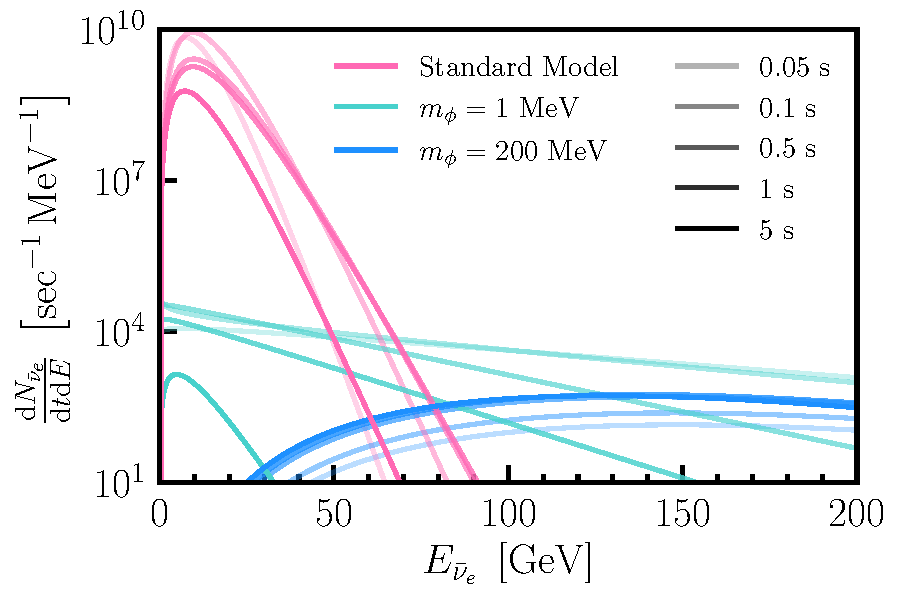
\includegraphics[width=0.47\textwidth]{figures/majoran_fluxes.pdf}
    \caption{\textbf{\textit{Neutrino flux from Standard Model production and two majoran hypotheses.}}
    Jeff needs to write here. {\color{red}also need to write the couplings used}
    }
    \label{fig:fluxes}
\end{figure}\\
